\section{Introduction}

% Two columns start
\iftwocolumns
\begin{multicols}{2}
\fi

This enters the discussion portion of the report. We will analyze the current processes in game development for UI/UX at BioWare. Then look at some of the more theoretical, template solutions known as design patterns in later sections and draw comparisons. We will also look into how the design patterns would be used in a general sense in game development (not specific to BioWare or Bioware's current project, Anthem).

\subsection{Game Development Overview}

% There are many parts to a video game. It can be grouped into: rendering, physics / simulation, AI, UI, sound / music. online, controls (input handling), online / networking. All tied together by the game engine.\\

% Having all the systems working together monolithically is bad, because it's difficult to maintain, prone to errors and bugs, and hard to collaborate as sub-systems are too tightly coupled.\\

% Talk about the video game industry -> video game development
% -> video game roles
A major portion of the video game market consists of AAA video games. These are titles with very high production value, large budget, and typically consists of a team of hundreds of developers. These developers consist of artists, scripters, programmers, managers, etc. Many of these roles are further grouped into sub-teams such as rendering, physics/simulation, AI, UI/UX, sound design, music production, networking, etc. Individual developers are specialized to work on one part of the game, with the exception of leads, managers, and other executives.

\subsubsection{Game Engine}
Developers will use a game engine so that many people can work on the project at once. The game engine is generally highly optimized for graphics rendering, physics simulation (such as collision detection), and object handling.\bs

The Frostbite engine is the game engine widely adopted at Electronic Arts (EA) studios. It was originally developed by Digital Illusions CE (DICE).\cite{frostbite}\cite{frostbite-wiki} As expected, the game engine is a piece of software, thus it is prone to software development problems that design patterns are ought to solve.

\subsection{Game Building}

Programmers make primitive entities such as an abstract UI widget, as well as the system that manages these entities.\bs
\\
The scripters and artists then use these entities in \textit{schematics} or \textit{blueprints}, which are used for visual scripting blocks of game content that contains logic and input/output together. Figure \ref{fig:unreal-blueprint} shows an example of what it looks like.\bs
\\
These schematics are in game levels, UI widgets, and prefabricated logic blocks (LogicPrefab). Thousands of these make up functionalities in a game, and are all handled by the game engine.

\begin{figure}[H]
	\centering
	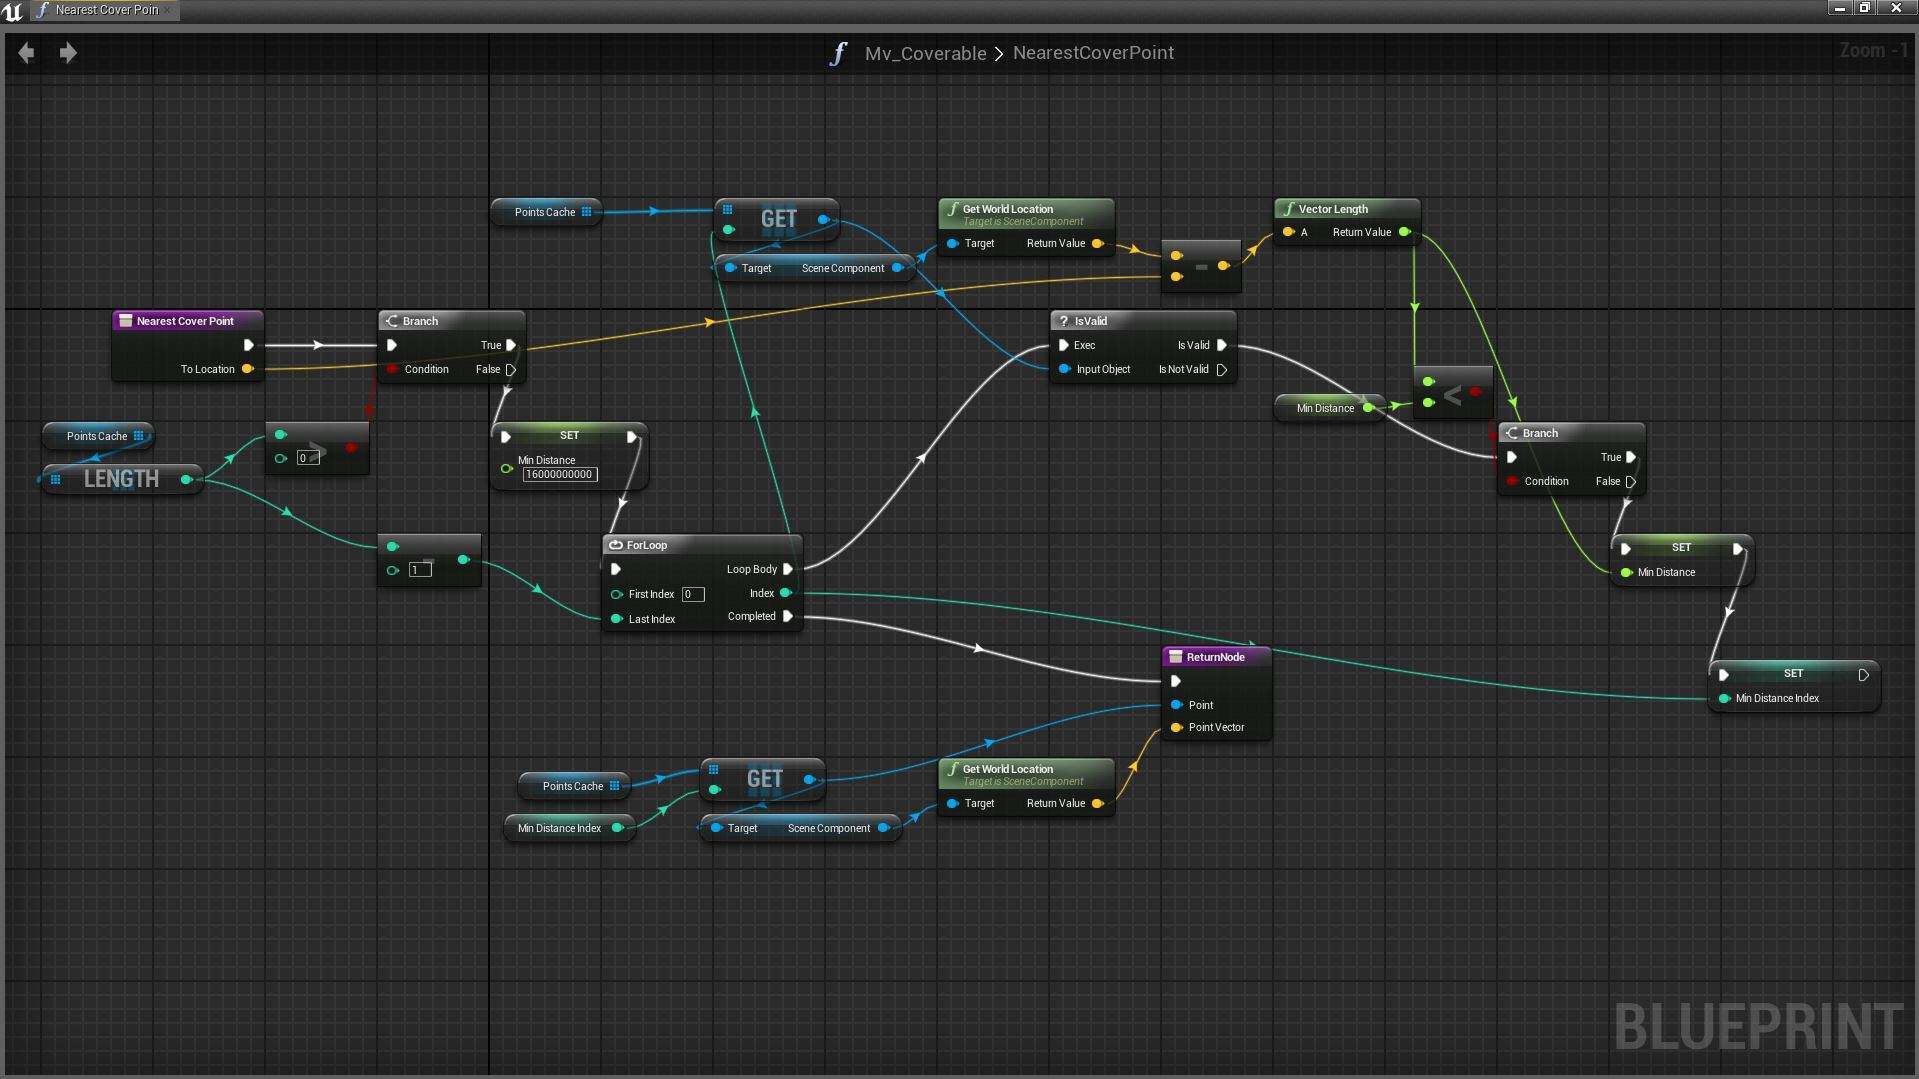
\includegraphics[width=0.49\textwidth]{assets/unreal-blueprint}
	\caption{Blueprint (schematics) for development in Unreal Engine\cite{unity-vs-unreal}}
	\label{fig:unreal-blueprint}
\end{figure}

\subsubsection{Role of Programmers}

At BioWare, most game programmers work with code (in C++ and C\#). Programmers are specialized to develop in-game entities, or tools for scripters, designers, and artists. Programmers also integrate systems together, such as making mouse inputs interact with hitzones widgets, which interacts with graphical widgets or animation timelines.\footnote{Animation timelines are timeline that describe how a particular object will animate. Example: a fade in.}

\subsection{Object Oriented Programming}

\textit{Object oriented programming} (OOP) is a programming paradigm centered around interaction of encapsulated objects. Objects have its own functions (methods), input and output (\textit(getters) and \textit(setters)), state and memory (member variables). OOP emphasizes on encapsulation which makes software structure easier to organize and debug. OOP allows programmers to define well-defined boundaries between features or objects. OOP also enables \textit{polymorphism} and \textit{inheritance} which are important in abstraction and organization of code.\cite{oop}\bs
\\
Although we will not go into depth into the subject of object oriented programming, it is vital to understand that OOP is basis of most modern game development due to its benefits of reusability, refactoring, extensibility/scalability, maintenance, and efficiency\cite{oop}. Nearly all of the design patterns explored here are utilizing OOP concepts in some way. 

\subsection{Design Pattern}

TODO:
Design patterns are reusable, general, abstract solutions to common problems in software development.\cite{sm-designpatterns} Design patterns are meant to be used when there no problems actually exist -- doing so would cause excess undesired complexity.\cite{gof}\bs
\\
Throughout the exploration in this report, we will see that all the patterns loosely fit into three categories of benefits: performance optimization, readability/maintainability improvement, organization/structure/scalability improvement. We use these three categories to evaluate the usefulness of the design patterns in game development. (TODO:)

\subsubsection{Antipatterns}
Software written without care are difficult to maintain, prone to bugs and errors, and hard to collaborate. Software written with these ``hacks'' are known as \textit{antipatterns}, where there is more negative consequences than the benefits of its solution. Antipatterns are counter parts to correctly implemented design patterns.\cite{sm-antipatterns}\bs
\\
Avoid antipatterns as much as possible. Exploring the negative effects of antipatterns is not part of the scope of this report.

\subsubsection{Gang of Four}

In software development, the phrase ``Gang of Four'' refers to the four authors of the Design Patterns book, Erich Gamma, Richard Helm, Ralph Johnson, and John Vlissides\cite{gof-wiki}\cite{gof}. The book features the most common design patterns widely in use today.\bs
\\
The design patterns featured in the book outlines the classical design patterns. Thus, many patterns would not be applicable as more recent revisions of programming languages (Python, C++11, etc.). This is because design patterns are inherently solutions / workarounds to limitations of the programming language. As there are more improvement in the usability of the language, certain design patterns (such as the \textit{template} pattern) are implemented less as it's less complex, less error prone, and easier to use the existing features built-in to a language.


% Two columns end
\iftwocolumns
\end{multicols}
\fi